\chapter{Design}
\label{ch:design}

The pipeline is designed to be able to take an image of a receipt sent over http as an input.
It is going to provide metadata to that image based on its contents.
This metadata includes the company name that issued the receipt, the date the receipt was made, and the price of the purchase.
In order to transfer the image to our machine learning models, a .NET API is used.

The pipeline consists of a website, .NET API, database, ML API, CNN, OCR and Spacy.

The webpage will take an image input from the user.
The webpage is connected with the .NET API and database.
From here the image is sent to a machine learning API\@.
This is written in java, we use it because we can't communicate directly to our python program with the .NET API\@.
The ML API is made by using a framework called Flask, this is used to convert the information to python and from here the image is sent to the CNN\@.

The CNN does a prediction on the category of the image.
Which is the company, this information is also returned to the API\@.
Since all the different companies got different receipts, we figured that this was the easiest way to do it.

For extracting the metadata for the companies we had one other solution that was heavily considered.
That was to not use a CNN, but rather have an RNN do all the predictions.
This would force us to change the alignment functionality of our pipeline.
The prediction will be sent to the OCR from the CNN and the image itself will already have been sent to the OCR from the API\@.
The prediction from the CNN will be used in the OCR to choose the right template for the image.
The template is an aligned image that we have pre-loaded into the OCR model.
This means that the OCR is holding one image of all the categorise we have and using this as a reference to skew the images horizontally (We need to do this because an OCR can't read skewed text).

The skewing method is using something called matching, this finds similarities in the images and aligns the images
based on these similarities. (You can read more about matching under implementation in chapter 4.5.1)
We have this feature because our sample size is way too small.
This forced us to create "fake" data by skewing images.
This is a feature that is great to have, but in reality, not needed.
This is because it is way better solutions for this.
We would add a check for the image before accepting it.
This would assure images that wasn't easily read by the OCR was discarded (the user would have to take another picture).

The aligned image is sendt to the second part of our OCR, where we do some simple thresholding and extracting the text from the image.
The OCR sends the extracted text as a string to the sapcy model and the date to the API\@.
The Spacy model reads the string, adds relations to the text and evaluates the what's the total price.
The date could also be evaluated in this model. (With research we have gotten the impression that its more common practise to find the date witn OCR).


Finally the data from CNN, OCR and Spacy is provided back to the user.
This pipeline is illustrated in figure~\ref{fig:pipeline}

\begin{figure}[h]
    \center{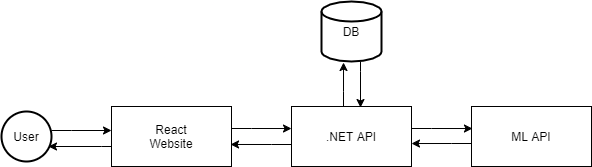
\includegraphics[width=1\textwidth]{Images/PipelineLess}}
    \caption{Graphic illustrating the project pipeline}
    \label{fig:pipeline}
\end{figure}

\begin{figure}[h]
    \center{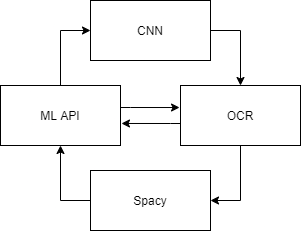
\includegraphics[width=0.5\textwidth]{Images/PipelineMLAPI.png}}
    \caption{ML API pipeline}
    \label{fig:ML API}
\end{figure}

\begin{figure}[h]
    \center{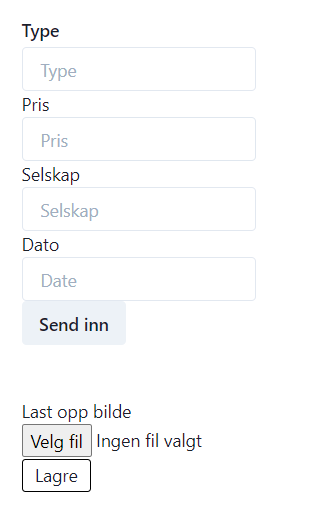
\includegraphics[width=0.5\textwidth]{Images/ReactWebsite.png}}
    \caption{React website}
    \label{fig:reactWebsite}
\end{figure}


\section{React website}\label{sec:reactWebsite}
The website is the first point in the pipeline and gives the user a way to interact with the pipeline.
The website allows the user to upload the picture which is sent through the pipeline, and consecutively the receipt (figure~\ref{fig:reactWebsite}).

\section{.NET API}\label{sec:.NET API}
The .NET API exposes several endpoints that allows for sending an image to the ML API, and save an image and a receipt to a database.

\section{ML API}\label{sec:ML API}
The ML API works as an endpoint for the machine learning model, it utilizes the CNN, OCR and Spacy to get data from
the image the user sends in, and then sends the data back to the .NET API\@.
The pipeline is explained in figure~\ref{fig:ML API}


\section{Dataset}\label{sec:dataset}
In order to train our neural network models, Simployer provided us with a sample of images from their database.
This dataset includes 1194 images of receipts taken with mobile cameras and generated pdfs from online sales.

\begin{figure}[h]
    \center{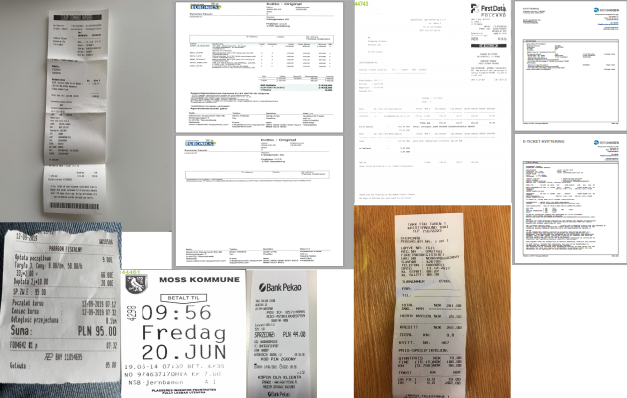
\includegraphics[width=1\textwidth]{Images/exampleimages_raw_resized}}
    \caption{Examples of the images found in the dataset provided by Simployer}
    \label{fig:figure3.2}
\end{figure}

This dataset is not labeled, which means we have to manually label the data we are going to use to train our networks.
Because of the large variance of different types of companies in this dataset, creating labels for all of them would be very time-consuming.
Instead of labeling them all, we decided to restrict ourselves to the three most common receipts found in the dataset.
This means the amount of images we can use for training is greatly reduced, so in order to combat this, we used data augmentation software to generate more images.
This is discussed in greater detail in chapter 4.

\section{Pre-processing}\label{sec:pre-processing}
A CNN does not require images of large resolution in order to accurately classify an image.
In addition, training the network with large resolution images take significantly longer.
Because of this, all the images that are going to be fed into the CNN are downscaled.
This also solves the problem of images being of different sizes, as the CNN requires all the images to have the same size.

\begin{figure}[h]
    \center{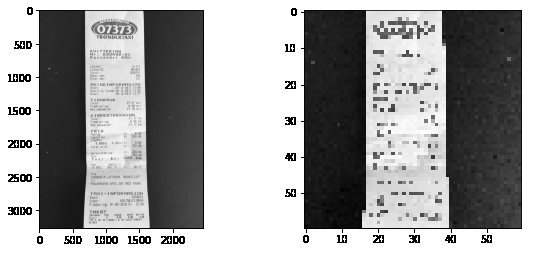
\includegraphics[width=1\textwidth]{Images/beforeafterrescale}}
    \caption{Before and after image rescaling}
    \label{fig:figure3.3}
\end{figure}
While the text in the image is now completely unreadable, the CNN will have no issues telling images in this format apart from each other.

\section{Convolutional Neural network}\label{sec:CNN}
As stated previously, we are using a CNN as an image classifier in order to determine which company issued the receipt.

\begin{figure}[h]
    \center{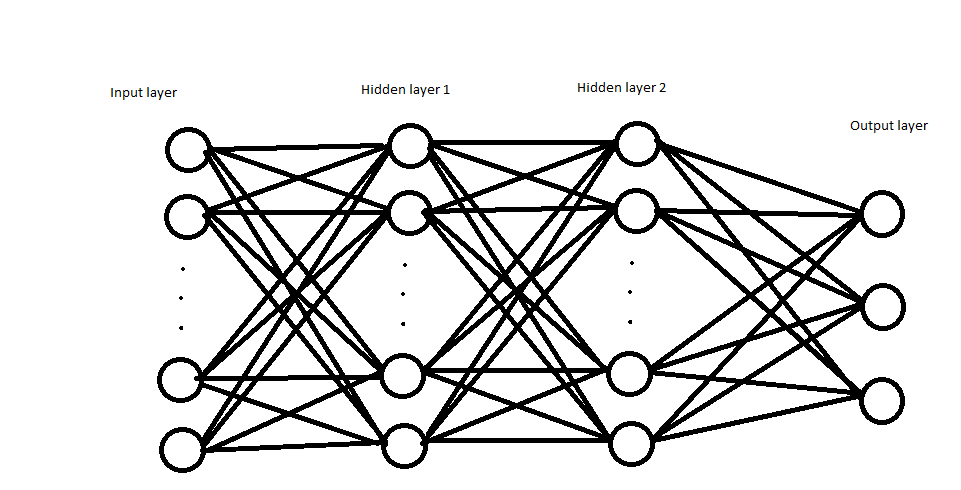
\includegraphics[width=1\textwidth]{Images/cnnplaceholder}}
    \caption{Graphic illustrating the Convolutional Neural Network (PLACEHOLDER)}
    \label{fig:cnnplaceholder.4}
\end{figure}

Figure 3.3 illustrates the layout of our CNN.
The input layer takes the pixel value of the image.
Because of this, the number of nodes in the input layer has to be equal to the amount of pixels in the image.
The output layer has three nodes, one for each type of receipt the network is trained to classify.

We are using a supervised learning-model to train our network.
Because of this, the training data has to be labeled.
This labeling can be labor intensive if the dataset you are labeling is large.
Since we started with a very small amount of images before the use of data augmentation, it is a small task.

\section{Optical Character Recognition}\label{sec:OCR}
In order to extract the text found in an image, we are using the open-source OCR software Python-tesseract.
Python-tesseract, or Pytesseract for short, utilizes Google's Tesseract-OCR engine.

When metadata for a particular image is requested by a user, the API will provide our implementation of Pytesseract with an image.
Pytesseract will take this image as an input, and can provide outputs in various formats like xml or pdf.
We will be using the output in string format, as this will serve as the input to our RNN model.
Once Pytesseract has completed the text extraction, the output string is then fetched by our API to be provided to our RNN model.

\begin{figure}[h]
    \center{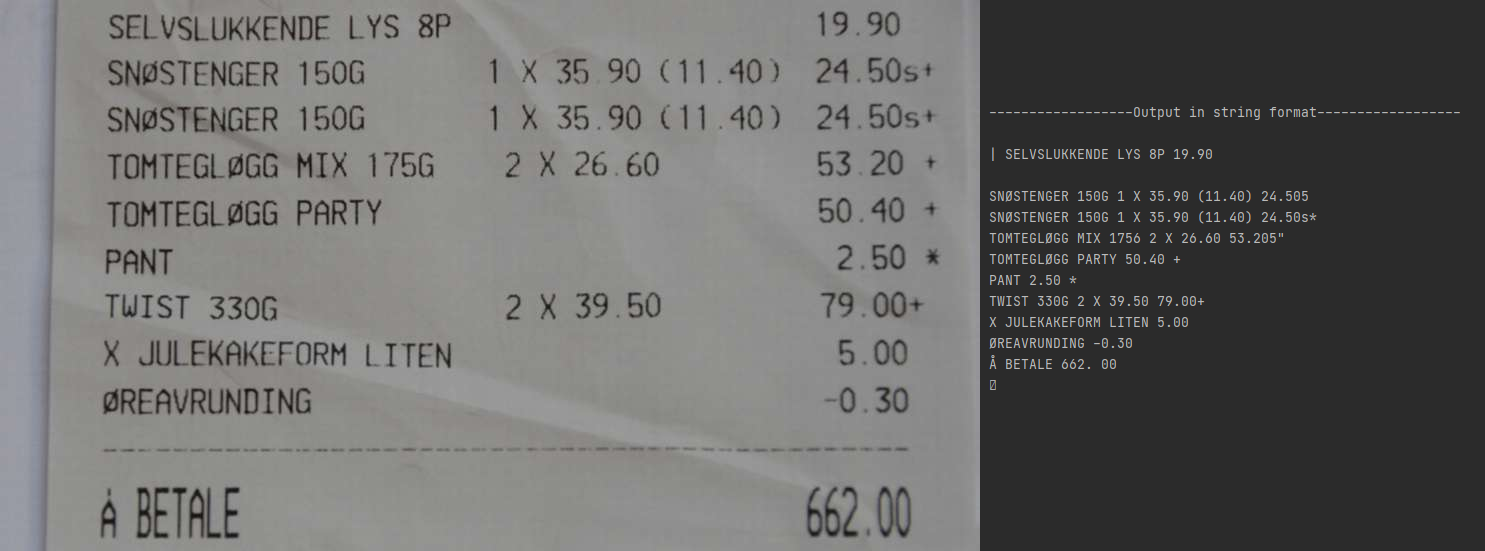
\includegraphics[width=1\textwidth]{Images/ocr_before_after}}
    \caption{Example output of pytesseract with a test image}
    \label{fig:figure3.5}
\end{figure}

\section{Recurrent Neural Network}\label{sec:RNN}

